\subsection{Angular}
Для выполнения работы потребовалось с фреймворком Angular по причине того, 
что веб-интерфейс пользователя был написан с использованием этой технологии.

Angular - это TypeScript-фреймворк с открытым исходным кодом, который 
предназначен для разработки одностраничных приложений. 
Цель фреймворка - расширение браузерных приложений на основе MVC-шаблона, 
а также упрощение разработки и тестирования.

Фреймворк работает с HTML, содержащим дополнительные пользовательские атрибуты, 
которые описываются директивами, и связывает ввод или вывод области страницы
с моделью, представляющей собой обычные переменные TypeScript. 
Значения этих переменных задаются 
вручную или извлекаются из статических или динамических JSON-данных.

Базовой единицей в данном фреймворке является компонент, который содержит
HTML шаблон, стили и логику в TypeScript файлах.

\vspace{2em}

\subsection{Markdown}

\vspace{1em}

Markdown — облегчённый язык разметки, созданный с целью написания
наиболее читаемого и удобного для правки текста, но пригодного для
преобразования в языки для продвинутых публикаций.

Markdown используется как язык разметки для статей базы знаний.

\vspace{2em}

\section{Расширение фунционала <<Базы знаний>>}

\vspace{1em}

\subsection{Изучение предметной области}

\vspace{1em}

База знаний в данной системе представлена списком статей в формате Markdown, 
который упрощает форматирование текста.
Изначально добавлять, редактировать статьи и их перевод 
мог только администратор, что накладывало на базу ряд ограничений: 
трудность поддержки актуальности статей, их качественное и количественное содержание.

Поэтому было решено разрешить пользователям предлагать свои правки и переводы
и, соответственно, добавить этот функционал в веб-интерфейс и сервер.

\vspace{1em}

\subsection{Добавление пользовательской формы для внесения правок}

\vspace{1em}

В качестве Markdown редактора был выбран SimpleMDE, так как он уже применялся в 
интерфейсе администратора для тех же целей.
Редактор доступен только авторизованным пользователям, которые нажали на соответствующую кнопку.
Если же пользователь не авторизован, то нужно показать форму входа, как на рисунке \ref{fig:user_sign_in}.

Также требуется реализовать возможность выбор языка локализации.

Примерный интерфейс пользователя представлен на рисунке \ref{fig:web_user_editor}.

\begin{figure}[!h]
    \centering
    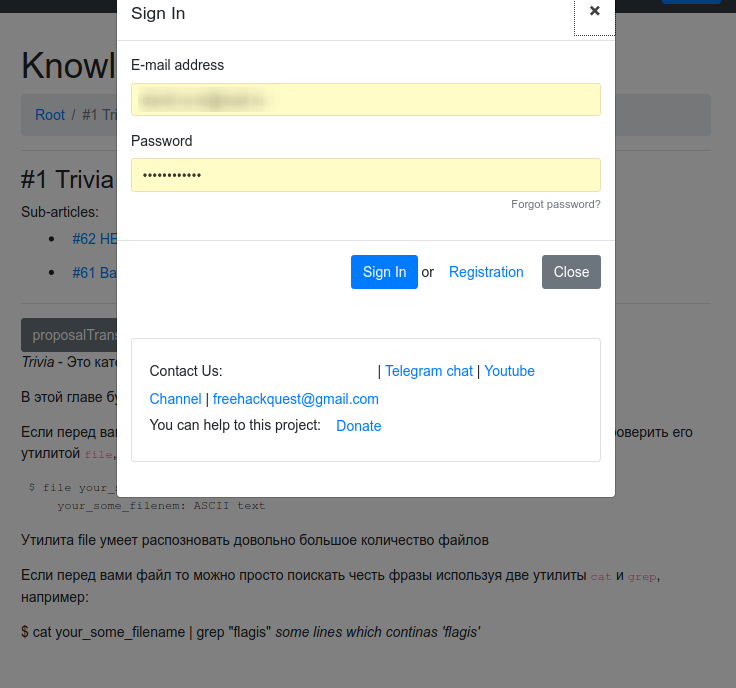
\includegraphics[width=0.6\linewidth]{images/user_sign_in.png}
    \caption{Форма входа}
    \label{fig:user_sign_in}
\end{figure}

\begin{figure}[!h]
    \centering
    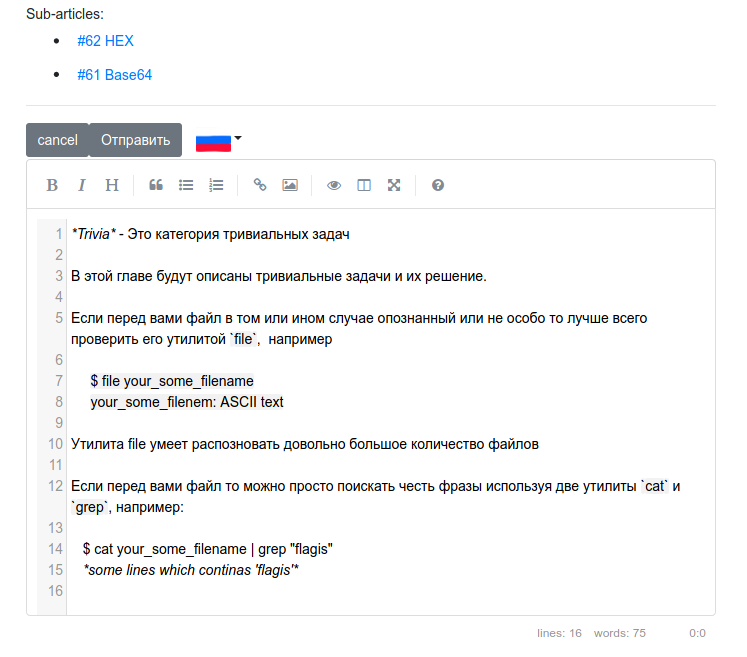
\includegraphics[width=0.6\linewidth]{images/user_web_editing.png}
    \caption{Интерфейс редактора}
    \label{fig:web_user_editor}
\end{figure}


По нажатию кнопки <<Отправить>> на сервер уходит запрос типа \\
\emph{classbook\_proposal\_add\_record}, в котором содержится
предлагаемое содержимое, язык, идентификатор статьи.

Если добавление правки в базу данных прошло успешно, 
то на веб-интерфейсе отобразится сообщение, показанное на рисунке \ref{fig:user_wait_msg}

\begin{figure}[!h]
    \centering
    
\includegraphics[width=0.6\linewidth]{images/user_wait_msg.png}
    \caption{Сообщение пользователю}
    \label{fig:user_wait_msg}
\end{figure}

\vspace{2em}

\subsection{Принятие и отклонение правок пользователей администратором}

Что касается интерфейса администратора, то нужно было добавить отображение списка правок
для данной статьи с отображением языка, возможностью редактировать, принять или отклонить правку.
Причём кнопка \emph{Approve} должна отображаться только для предложений.

Новый интерфейс администратора представлен на рисунке \ref{fig:admin_web_editing}.

\begin{figure}[!h]
    \centering
    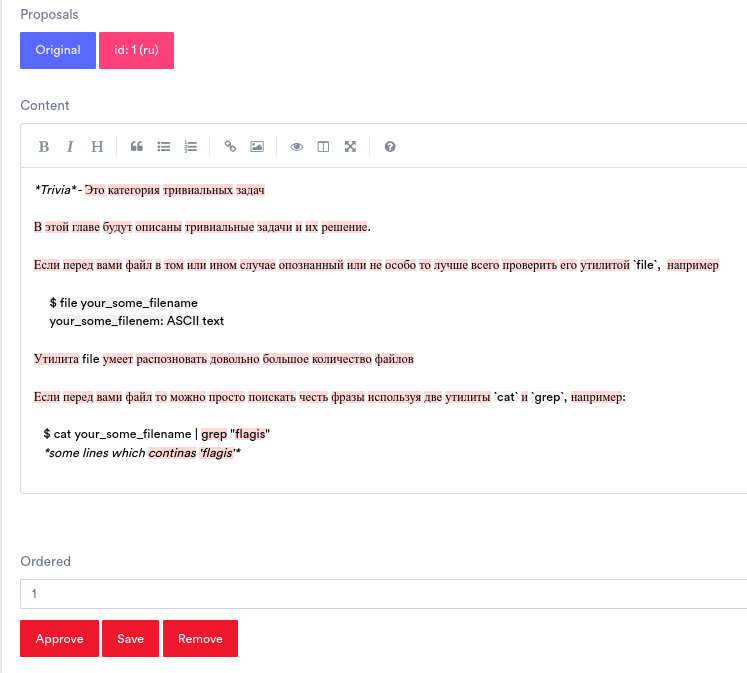
\includegraphics[width=0.6\linewidth]{images/admin_web_editing.png}
    \caption{Интерфейс администратора}
    \label{fig:admin_web_editing}
\end{figure}

Текущий выбор варианта статьи (оригинал или правка) для
редактирования отображается другим цветом (розовым в данном случае) в списке <<Propasals>>.

Данный список подгружает с сервера запросом \emph{classbook\_proposal\_list}, который принимает идентификатор статьи.

Кнопка <<Approve>> отвечает за принятие правки, с помощью запроса \emph{classbook\_proposal\_approve}.

Кнопка <<Save>> обновляет предложение или оригинальную статью, с помощью запроса \emph{classbook\_proposal\_update} или \emph{classbook\_update\_record} соответственно.

Кнопка <<Remove>> удаляет предложение или статью вообще, с помощью запроса \emph{classbook\_proposal\_remove} или \emph{classbook\_remove\_record} соответственно.

\vspace{2em}

\subsection{Серверная часть}

\vspace{1em}

Для функционала, описанного выше, были добавлены 2 новых типа запроса: \\ 
\emph{classbook\_proposal\_approve} и \emph{classbook\_proposal\_update}.
Оба принимают идентификатор правки, а второе ещё и новое содержимое.

Структура базы данных, охватывающая 3 таблицы: \emph{classbook}, \\ 
\emph{classbook\_proposal}, \emph{classbook\_localization}, представлена на рисунке \ref{fig:db_classbook}.

\begin{figure}[!h]
    \centering
    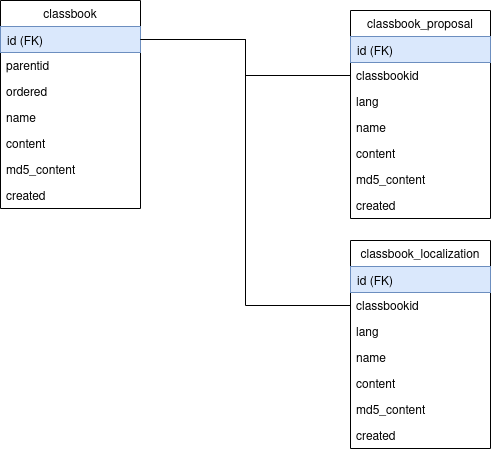
\includegraphics[width=0.6\linewidth]{images/db_classbook.png}
    \caption{Структура базы данных}
    \label{fig:db_classbook}
\end{figure}

В \emph{classbook} хранятся метаинформация о статье (родительская статья, позиция, 
дата создания, md5 от контента) и само содержимое (имя, контент).

В \emph{classbook\_localization} хранятся данные локализации(язык, имя, контент)
и отношения к оригинальной статье (идентификатор статьи).

В \emph{classbook\_proposal} хранятся правка (язык, имя, контент) и само содержимое (имя, контент).

В \emph{classbook\_proposal\_approve} нужно получить идентификатор правки и найти саму статью, 
код на рисунке \ref{fig:code_classbook_id} реализует это.

\begin{figure}[!h]
    \centering
    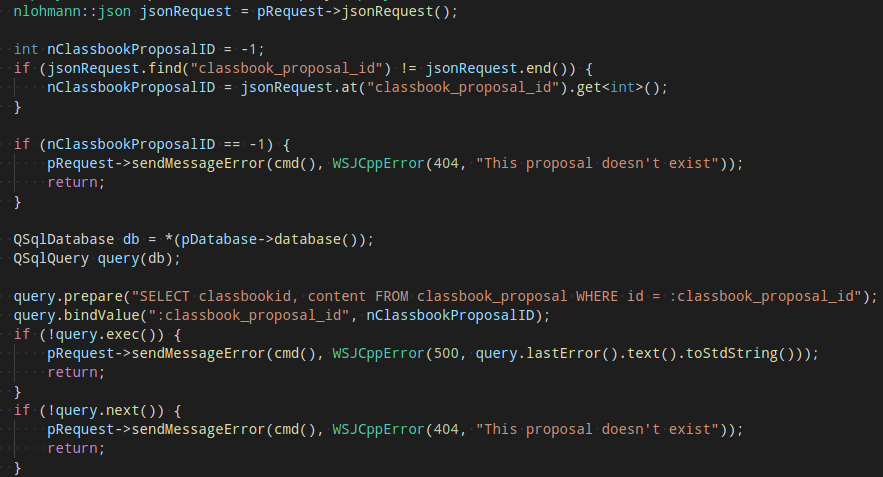
\includegraphics[width=0.8\linewidth]{images/code_classbook_id.png}
    \caption{Получение идентификатора статьи}
    \label{fig:code_classbook_id}
\end{figure}

В зависимости от языка происходит выбор в какую таблицу производить запись, 
код на рисунке \ref{fig:code_update_classbook} производит запись в таблицу \emph{classbook},
если язык правки - русский:

\begin{figure}[!h]
    \centering
    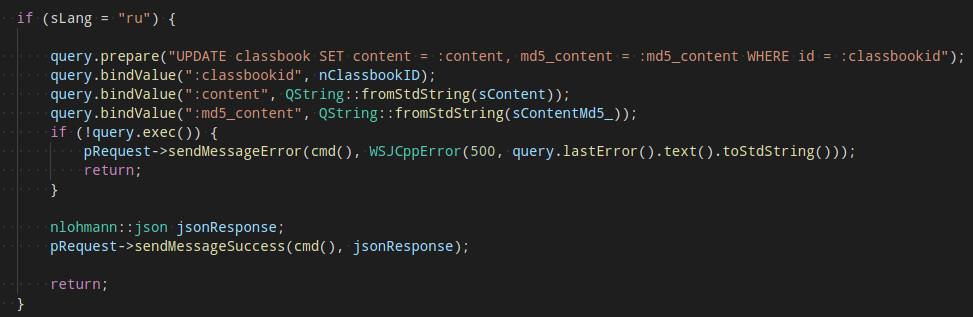
\includegraphics[width=0.8\linewidth]{images/code_update_classbook.png}
    \caption{Обновление статьи}
    \label{fig:code_update_classbook}
\end{figure}

Обновление правки в запросе \emph{classbook\_proposal\_update} происходит в 2 этапа:
\begin{itemize}
    \item Валидация входных данных - не отличается от соответствующего кода в предыдущем запросе.
    \item Запись в БД, которая представлена на рисунке \ref{fig:proposal_update}
\end{itemize}

\begin{figure}[!h]
    \centering
    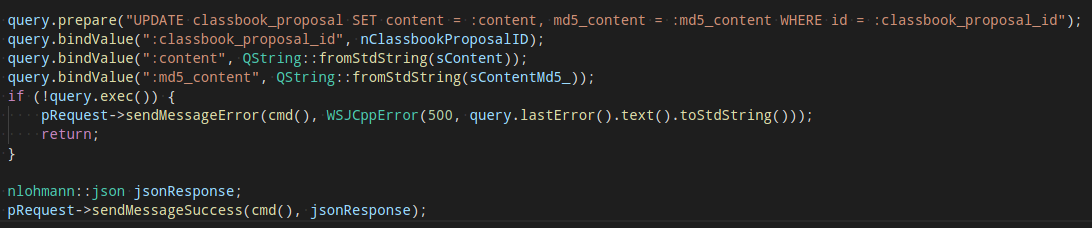
\includegraphics[width=0.8\linewidth]{images/proposal_update.png}
    \caption{Обновление правки}
    \label{fig:proposal_update}
\end{figure}